\documentclass[12pt,fleqn]{article}\usepackage{../../common}
\begin{document}
Tam Varyasyon ile G�r�lt� ��kartmak (Total Variation Denoising)

\begin{minted}[fontsize=\footnotesize]{python}
f = 'xcor.mat'
import scipy.io as sio
xcor = sio.loadmat(f)
xcor = xcor['xcor']
xcor = np.reshape(xcor,(len(xcor)))
plt.plot(range(len(xcor)), xcor)
plt.savefig('func_60_tvd_01.png')
\end{minted}

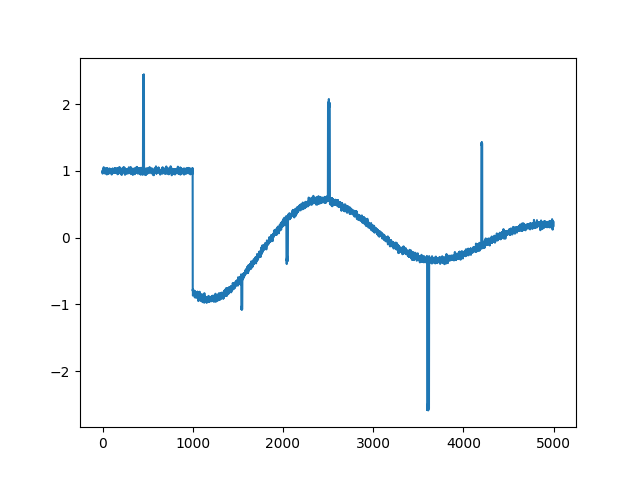
\includegraphics[width=25em]{func_60_tvd_01.png}

\begin{minted}[fontsize=\footnotesize]{python}
import numpy as np

eps = 1e-6
mu = 50.0

def phi_tv(x):
   return np.sum(np.abs(np.diff(x)))
   
def phi_atv(x):
   return np.sum(np.sqrt(eps + np.power(np.diff(x),2)) - eps)
   
def f(u):
   return np.sum(np.power(u-xcor, 2)) + mu*phi_atv(u)

print (phi_tv(xcor))
print (phi_atv(xcor))
\end{minted}

\begin{verbatim}
155.63025715999999
155.8936302273509
\end{verbatim}


\begin{minted}[fontsize=\footnotesize]{python}
u0 = np.zeros(len(xcor))
print (f(u0))

from scipy.optimize import minimize, Bounds, SR1, BFGS

opts = {'maxiter': 400, 'verbose': 2}

res = minimize (fun=f,
                x0=u0,
                options=opts,
                jac='2-point',
                hess=BFGS(),
                method='trust-constr'
                )

plt.plot(range(5000), res.x)
plt.savefig('')
\end{minted}

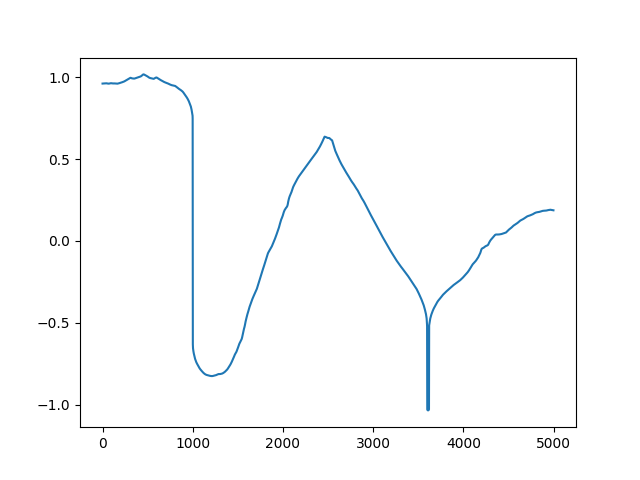
\includegraphics[width=25em]{func_60_tvd_02.png}


\begin{minted}[fontsize=\footnotesize]{python}
import pandas as pd
import scipy.sparse as sps
import scipy.sparse.linalg as slin

df = pd.read_csv('xcor.csv',header=None)
xcor = np.reshape(np.array(df[0]), (5000,1))
MU = 50.0
EPSILON = 0.001

ALPHA = 0.01;
BETA = 0.5;
MAXITERS = 100;
NTTOL = 1e-10;

n = len(xcor)
data = np.array([-1*np.ones(n), np.ones(n)])
diags = np.array([0, 1])
D = sps.spdiags(data, diags, n-1, n)

x = np.zeros((len(xcor),1))

for iter in range(MAXITERS):
   d = D.dot(x)
   tmp1 = np.dot((x-xcor).T,(x-xcor))
   tmp2a = np.sqrt(EPSILON**2 + np.power(d,2))
   tmp2b = EPSILON*np.ones((n-1,1))
   val = np.float(tmp1 + MU*np.sum(tmp2a - tmp2b))
   tmp1 = 2*(x-xcor)
   tmp2 = MU*D.T.dot(d / np.sqrt(EPSILON**2 + d**2))
   grad = tmp1 + tmp2
   tmp1 = 2*sps.eye(n)
   tmp2 = EPSILON**2*(EPSILON**2+d**2)**(-3/2)
   tmp2 = tmp2.reshape((n-1))
   tmp3 = sps.spdiags(tmp2, 0, n-1, n-1)

   hess = tmp1 + MU*tmp3.dot(D).T.dot(D)
   v = slin.spsolve(-hess, grad)
   v = np.reshape(v, (n,1))
   lambdasqr = np.float(np.dot(-grad.T,v))
   if lambdasqr/2 < NTTOL: break
   t = 1;
   while True:
      tmp1 = np.float(np.dot((x+t*v-xcor).T,(x+t*v-xcor)))
      tmp2 = MU*np.sum(np.sqrt(EPSILON**2+(D*(x+t*v))**2)-EPSILON*np.ones((n-1,1)))
      tmp3 = val - ALPHA*t*lambdasqr
      if tmp1 + tmp2 < tmp3: break
      t = BETA*t

   x = x+t*v
\end{minted}



Kaynaklar

[1] {\em ROF and TV-L1 denoising with Primal-Dual algorithm}, 
    \url{https://github.com/znah/notebooks/blob/master/TV_denoise.ipynb}

[2] {\em An introduction to continuous optimization for imaging}, 
    \url{https://hal.archives-ouvertes.fr/hal-01346507/document}

\end{document}



